\documentclass[12pt]{article}
\usepackage[left=1cm, right=1cm, top=2cm,bottom=1.5cm]{geometry} 

\usepackage[parfill]{parskip}
\usepackage[utf8]{inputenc}
\usepackage[T2A]{fontenc}
\usepackage[russian]{babel}
\usepackage{enumitem}
\usepackage[normalem]{ulem}
\usepackage{amsfonts, amsmath, amsthm, amssymb, mathtools,xcolor}
\usepackage{blkarray}

\usepackage{tabularx}
\usepackage{hhline}

\usepackage{accents}
\usepackage{fancyhdr}
\pagestyle{fancy}
\renewcommand{\headrulewidth}{1.5pt}
\renewcommand{\footrulewidth}{1pt}

\usepackage{graphicx}
\usepackage[figurename=Рис.]{caption}
\usepackage{subcaption}
\usepackage{float}

%%Наименование папки откуда забирать изображения
\graphicspath{ {./images/} }

%%Изменение формата для ввода доказательства
\renewcommand{\proofname}{$\square$  \nopunct}
\renewcommand\qedsymbol{$\blacksquare$}

%%Изменение отступа на таблицах
\addto\captionsrussian{%
	\renewcommand{\proofname}{$\square$ \nopunct}%
}
%% Римские цифры
\newcommand{\RN}[1]{%
	\textup{\uppercase\expandafter{\romannumeral#1}}%
}

%% Для удобства записи
\newcommand{\MR}{\mathbb{R}}
\newcommand{\MC}{\mathbb{C}}
\newcommand{\MQ}{\mathbb{Q}}
\newcommand{\MN}{\mathbb{N}}
\newcommand{\MZ}{\mathbb{Z}}
\newcommand{\MTB}{\mathbb{T}}
\newcommand{\MTI}{\mathbb{I}}
\newcommand{\MI}{\mathrm{I}}
\newcommand{\MCI}{\mathcal{I}}
\newcommand{\MJ}{\mathrm{J}}
\newcommand{\MH}{\mathrm{H}}
\newcommand{\MT}{\mathrm{T}}
\newcommand{\MU}{\mathcal{U}}
\newcommand{\MV}{\mathcal{V}}
\newcommand{\MB}{\mathcal{B}}
\newcommand{\MF}{\mathcal{F}}
\newcommand{\MW}{\mathcal{W}}
\newcommand{\ML}{\mathcal{L}}
\newcommand{\MP}{\mathcal{P}}
\newcommand{\VN}{\varnothing}
\newcommand{\VE}{\varepsilon}
\newcommand{\dx}{\, dx}
\newcommand{\dy}{\, dy}
\newcommand{\dz}{\, dz}
\newcommand{\dd}{\, d}


\theoremstyle{definition}
\newtheorem{defn}{Опр:}
\newtheorem{rem}{Rm:}
\newtheorem{prop}{Утв.}
\newtheorem{exrc}{Упр.}
\newtheorem{problem}{Задача}
\newtheorem{lemma}{Лемма}
\newtheorem{theorem}{Теорема}
\newtheorem{corollary}{Следствие}

\newenvironment{cusdefn}[1]
{\renewcommand\thedefn{#1}\defn}
{\enddefn}

\DeclareRobustCommand{\divby}{%
	\mathrel{\text{\vbox{\baselineskip.65ex\lineskiplimit0pt\hbox{.}\hbox{.}\hbox{.}}}}%
}
\DeclareRobustCommand{\ndivby}{\mkern-1mu\not\mathrel{\mkern4.5mu\divby}\mkern1mu}


%Короткий минус
\DeclareMathSymbol{\SMN}{\mathbin}{AMSa}{"39}
%Длинная шапка
\newcommand{\overbar}[1]{\mkern 1.5mu\overline{\mkern-1.5mu#1\mkern-1.5mu}\mkern 1.5mu}
%Функция знака
\DeclareMathOperator{\sgn}{sgn}

%Функция ранга
\DeclareMathOperator{\rk}{\text{rk}}
\DeclareMathOperator{\diam}{\text{diam}}


%Обозначение константы
\DeclareMathOperator{\const}{\text{const}}

\DeclareMathOperator{\codim}{\text{codim}}

\DeclareMathOperator*{\dsum}{\displaystyle\sum}
\newcommand{\ddsum}[2]{\displaystyle\sum\limits_{#1}^{#2}}

%Интеграл в большом формате
\DeclareMathOperator{\dint}{\displaystyle\int}
\newcommand{\ddint}[2]{\displaystyle\int\limits_{#1}^{#2}}
\newcommand{\ssum}[1]{\displaystyle \sum\limits_{n=1}^{\infty}{#1}_n}

\newcommand{\smallerrel}[1]{\mathrel{\mathpalette\smallerrelaux{#1}}}
\newcommand{\smallerrelaux}[2]{\raisebox{.1ex}{\scalebox{.75}{$#1#2$}}}

\newcommand{\smallin}{\smallerrel{\in}}
\newcommand{\smallnotin}{\smallerrel{\notin}}

\newcommand*{\medcap}{\mathbin{\scalebox{1.25}{\ensuremath{\cap}}}}%
\newcommand*{\medcup}{\mathbin{\scalebox{1.25}{\ensuremath{\cup}}}}%

\makeatletter
\newcommand{\vast}{\bBigg@{3.5}}
\newcommand{\Vast}{\bBigg@{5}}
\makeatother

%Промежуточное значение для sup\inf, поскольку они имеют разную высоту
\newcommand{\newsup}{\mathop{\smash{\mathrm{sup}}}}
\newcommand{\newinf}{\mathop{\mathrm{inf}\vphantom{\mathrm{sup}}}}

%Скалярное произведение
\newcommand{\inner}[2]{\left\langle #1, #2 \right\rangle }
\newcommand{\linsp}[1]{\left\langle #1 \right\rangle }
\newcommand{\linmer}[2]{\left\langle #1 \vert #2\right\rangle }

%Подпись символов снизу
\newcommand{\ubar}[1]{\underaccent{\bar}{#1}}

%% Шапка для букв сверху
\newcommand{\wte}[1]{\widetilde{#1}}
\newcommand{\wht}[1]{\widehat{#1}}
\newcommand{\ovl}[1]{\overline{#1}}

%%Трансформация Фурье
\newcommand{\fourt}[1]{\mathcal{F}\left(#1\right)}
\newcommand{\ifourt}[1]{\mathcal{F}^{-1}\left(#1\right)}

%%Символ вектора
\newcommand{\vecm}[1]{\overrightarrow{#1\,}}

%%Пространстов матриц
\newcommand{\matsq}[1]{\operatorname{Mat}_{#1}}
\newcommand{\mat}[2]{\operatorname{Mat}_{#1, #2}}

%Оператор для действ и мнимых чисел
\DeclareMathOperator{\IM}{\operatorname{Im}}
\DeclareMathOperator{\RE}{\operatorname{Re}}
\DeclareMathOperator{\li}{\operatorname{li}}
\DeclareMathOperator{\GL}{\operatorname{GL}}
\DeclareMathOperator{\SL}{\operatorname{SL}}
\DeclareMathOperator{\Char}{\operatorname{char}}

%Делимость чисел
\newcommand{\modn}[3]{#1 \equiv #2 \; (\bmod \; #3)}


%%Взятие в скобки, модули и норму
\newcommand{\parfit}[1]{\left( #1 \right)}
\newcommand{\modfit}[1]{\left| #1 \right|}
\newcommand{\sqparfit}[1]{\left\{ #1 \right\}}
\newcommand{\normfit}[1]{\left\| #1 \right\|}

%%Функция для обозначения равномерной сходимости по множеству
\newcommand{\uconv}[1]{\overset{#1}{\rightrightarrows}}
\newcommand{\uconvm}[2]{\overset{#1}{\underset{#2}{\rightrightarrows}}}


%%Функция для обозначения нижнего и верхнего интегралов
\def\upint{\mathchoice%
	{\mkern13mu\overline{\vphantom{\intop}\mkern7mu}\mkern-20mu}%
	{\mkern7mu\overline{\vphantom{\intop}\mkern7mu}\mkern-14mu}%
	{\mkern7mu\overline{\vphantom{\intop}\mkern7mu}\mkern-14mu}%
	{\mkern7mu\overline{\vphantom{\intop}\mkern7mu}\mkern-14mu}%
	\int}
\def\lowint{\mkern3mu\underline{\vphantom{\intop}\mkern7mu}\mkern-10mu\int}

%%След матрицы
\DeclareMathOperator*{\tr}{tr}

\makeatletter
\renewcommand*\env@matrix[1][*\c@MaxMatrixCols c]{%
	\hskip -\arraycolsep
	\let\@ifnextchar\new@ifnextchar
	\array{#1}}
\makeatother


%% Переопределение функции хи, чтобы выглядела более приятно
\makeatletter
\@ifdefinable\@latex@chi{\let\@latex@chi\chi}
\renewcommand*\chi{{\@latex@chi\smash[t]{\mathstrut}}} % want only bottom half of \mathstrut
\makeatletter

\begin{document}
\lhead{Алгебра-\RN{1}}
\chead{Тимашев Д.А.}
\rhead{Лекция - 12}
\section*{Кольца вычетов}

\begin{defn}
	\uwave{Сравнимость} целых чисел по модулю $m \in \MN$: $\modn{k}{l}{m}$, если $k - l \divby m$ (то есть разность чисел $k-l$ делится на $m$). Эквивалентным образом: $k$ и $l$ имеют одинаковые остатки при делении на $m$.
\end{defn}

\begin{defn}
	\uwave{Класс вычетов} числа $k \in \MZ$ по модулю $m$ (\uwave{вычет числа} $k$ по модулю $m$) это множество:
	$$
		k \; \bmod \; m = \{l \in \MZ \colon \modn{l}{k}{m}\} = \{l = k + m{\cdot}n \colon n \in \MZ\} = k + m{\cdot}\MZ
	$$
	где $m{\cdot}\MZ$ - это множество всех целых чисел кратных $m$.
\end{defn}
\textbf{\uline{Обозначение}}: $k \; \bmod \; m = \ovl{k}$.

\subsection*{Основные свойства классов вычетов}
\begin{enumerate}[label=\arabic*)]
	\item В одном классе вычетов все числа сравнимы между собой по модулю $m$, поскольку имеют один и тот же остаток при делении на $m$;
	\item Числа из разных классов вычетов несравнимы по модулю $m$, поскольку имеют разные остатки при делении на $m$;
	\item Разные классы вычетов между собой не пересекаются;
	\item Любое целое число попадает в какой-то класс вычетов, то есть все классы вычетов по модулю $m$ образуют разбиение $\MZ$ на попарно непересекающиеся подмножества;
\end{enumerate}

\uline{Множество классов вычетов} по модулю $m$ обозначается как $\MZ_m = \left\{\ovl{0},\ovl{1},\ovl{2},\dotsc, \ovl{m-1}\right\}$. Графически это множество можно представить так:
\begin{figure}[H]
	\centering
	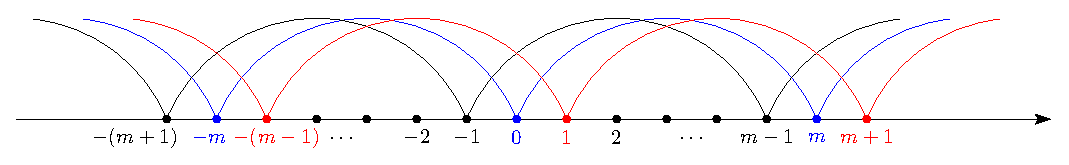
\includegraphics[width=0.9\textwidth]{AL1L12_1.eps}
	\caption{Геометрическое изображение классов вычетов.}
	\label{12_1}
\end{figure}
Или же ``свернуть'' в окружность длины $m$, то тогда все элементы из одного и того же класса вычетов попадут в одну и ту же точку на окружности:
\begin{figure}[H]
	\centering
	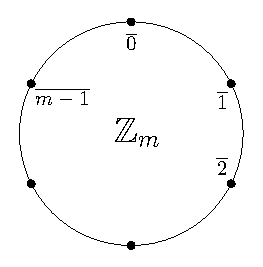
\includegraphics[width=0.27\textwidth]{AL1L12_2.eps}
	\caption{Геометрическое изображение классов вычетов в виде окружности.}
	\label{12_2}
\end{figure}
Таким образом, прямая превратилась в окружность. Точка $\ovl{0}$ - класс вычетов нуля и так далее до класса $\ovl{m-1}$, а дальше снова вернемся в класс вычетов $\ovl{0}$. Таким образом, разумнее изображать точками на окружности, плюс отсюда становится ближе терминология кольца вычетов.

\begin{defn}
	Определим \uwave{операции над вычетами} следующим образом:
	\begin{enumerate}[label =\arabic*)]
		\item \textbf{Сумма вычетов}: $\ovl{k} + \ovl{l} = \ovl{k+l}$;
		\item \textbf{Произведение вычетов}: $\ovl{k}{\cdot}\ovl{l} = \ovl{k{\cdot}l}$;
	\end{enumerate}
\end{defn}

\begin{prop}(\textbf{Корректность определения})
	Операции над вычетами определены однозначно (то есть не зависят от выбора представителей классов вычетов).
\end{prop}
\begin{proof}
	Пусть $k' \equiv k, \, l' \equiv l \Rightarrow k' = k + m{\cdot}r, \, l' = l +m{\cdot}s$, тогда: 
	\begin{enumerate}[label =\arabic*)]
		\item $k' + l' = k + l + m{\cdot}(r + s) \equiv k + l$;
		\item $k'{\cdot}l' = k{\cdot}l + m{\cdot}r{\cdot}l + k{\cdot}m{\cdot}s + m^2{\cdot}r{\cdot}s = k{\cdot}l + m{\cdot}(r{\cdot}l + k{\cdot}s + m{\cdot}r{\cdot}s) \equiv k{\cdot}l$;
	\end{enumerate}
\end{proof}

\textbf{Пример}: Рассмотрим $\MZ_5 =\left\{\ovl{0}, \ovl{1}, \ovl{2}, \ovl{3}, \ovl{4}\right\}$: $\ovl{3} + \ovl{4} = \ovl{7} = \ovl{2}, \, \ovl{3}{\cdot}\ovl{2} = \ovl{6} = \ovl{1}$.

Свойства операций в $\MZ_m$ определяются свойствами операций в $\MZ$. В частности из этих свойств вытекает, что $\MZ_n$ - коммутативное, ассоциативное кольцо с единицей (\uwave{кольцо вычетов по модулю} $m$).

Отметим, что в кольце целых чисел нет делителей нуля, тогда как в кольце вычетов они могут быть.

\textbf{Пример}: Рассмотрим $\MZ_6$: $\ovl{3}{\cdot}\ovl{2} = \ovl{0}$, то есть в кольце вычетов могут быть делители нуля.

\begin{prop}
	Для делителей нуля кольца вычетов $\MZ_m$ будет верно следующее:
	\begin{enumerate}[label=\arabic*)]
		\item $\ovl{k} \in \MZ_m$ - делитель нуля $\Leftrightarrow k \ndivby m$ и $k,m$ - имеют общие делители больше $1$;
		\item $\ovl{k} \in \MZ_m^{\times} \Leftrightarrow k,m$ - взаимно просты, то есть не имеют общих делителей больших $1$;
	\end{enumerate}
\end{prop}
\begin{rem}
	Из утверждения видно, что любой элемент кольца вычетов это либо ноль, либо делитель нуля, либо обратимый элемент.
\end{rem}
\begin{proof}\hfill
	\begin{enumerate}[label=\arabic*)]
		\item $(\Rightarrow)$ $\ovl{k}$ - делитель нуля $\Leftrightarrow \ovl{k} \neq \ovl{0} \wedge \exists\, \ovl{l} \neq 0 \colon \ovl{k}{\cdot}\ovl{l} = \ovl{0}$. Переформулируем эти свойства:
		$$
			\ovl{k} \neq \ovl{0} \Leftrightarrow k \ndivby m
		$$
		$$
			\exists\, \ovl{l} \neq 0 \colon \ovl{k}{\cdot}\ovl{l} = \ovl{0} \Leftrightarrow \exists \, l \ndivby m \colon k{\cdot}l \divby m \Rightarrow (k,m) > 1 
		$$
		то есть $k$ и $m$ имеют общие делители больше $1$. Если бы $k$ не имело общих делителей с $m$, а произведение делилось бы на $m$, то $l \divby m$, что не так по условию. 
		
		$(\Leftarrow)$ Пусть верно:
		$$
			k \ndivby m, \, k = k'{\cdot}d, \, m = m'{\cdot}d, \, m > d = (k,m) > 1
		$$
		Возьмем $l = m' < m$, тогда $k{\cdot}l = k'{\cdot}d{\cdot}m' = k'{\cdot}m \Rightarrow k{\cdot} l \divby m \Rightarrow \ovl{k}$ - делитель нуля;
		\item $(\Rightarrow)$ $\ovl{k} \in \MZ_m^{\times} \Rightarrow \ovl{k} \neq \ovl{0} \wedge \ovl{k}$ - неделитель нуля (т.к. они необратимы) $\Leftrightarrow k \ndivby m \wedge (k,m) = 1$, то есть числа $k$ и $m$ не имеют общих делителей больше $1 \Leftrightarrow$ $k$ и $m$ - взаимно просты. 
		
		$(\Leftarrow)$ Пусть верно: $\ovl{k} \neq \ovl{0}$ и $\ovl{k}$ - неделитель нуля. Рассмотрим множество произведений: 
		$$
			\left\{\ovl{k}{\cdot}\ovl{0},   \ovl{k}{\cdot}\ovl{1},  \ovl{k}{\cdot}\ovl{2}, \dotsc, \ovl{k}{\cdot}\ovl{m-1} \right\}
		$$
		таких произведений будет $m$ штук. Более того, $\ovl{k}{\cdot}\ovl{i} = \ovl{k}{\cdot}\ovl{j} \Rightarrow \ovl{i} = \ovl{j}$, поскольку на неделители нуля можно сокращать. Следовательно, все такие произведения будут различными и верно равенство:
		$$
			\left\{\ovl{k}{\cdot}\ovl{0},   \ovl{k}{\cdot}\ovl{1},  \ovl{k}{\cdot}\ovl{2}, \dotsc, \ovl{k}{\cdot}\ovl{m-1} \right\} = \left\{\ovl{0},\ovl{1},\ovl{2}, \dotsc ,\ovl{m-1}\right\}
		$$
		В частности, $\exists\, \ovl{l} \in \MZ_m \colon \ovl{k}{\cdot}\ovl{l} =\ovl{1} \Rightarrow \ovl{k}$ - обратим;
	\end{enumerate}
\end{proof}

\begin{corollary}
	$\MZ_m$ - поле $\Leftrightarrow m$ - простое число.
\end{corollary}

\begin{proof}
	$\MZ_m$ - поле $\Leftrightarrow \MZ_m^{\times} = \MZ_m \setminus \{\ovl{0}\} \Leftrightarrow \forall k = 1,2, \dotsc, m-1 $ - взаимно просты с $m$, то есть $(m,k) = 1$. Это как раз и означает, что $m$ - простое число.
\end{proof}

\textbf{Пример}: $\MZ_5 = \{\ovl{0},\ovl{1},\ovl{2},\ovl{3},\ovl{4}\}$ является полем.

\begin{prop}
	В $\MZ_m$ верно свойство: $\underbrace{\ovl{1} + \ovl{1} + \dotsc + \ovl{1}}_{m} = \ovl{0}$. 
\end{prop}
\begin{proof}
	Очевидно: $\underbrace{\ovl{1} + \ovl{1} + \dotsc + \ovl{1}}_{m} = \ovl{m} = \ovl{0}$.
\end{proof}
Это необычное для полей свойство, например в $\MR$ сложение единиц бесконечно растёт.

\begin{defn}
	Пусть $K$ - произвольное поле, назовем его \uwave{характеристикой} $\Char{K}$ наименьшее число $p \in \MN$ такое, что: $\underbrace{1 + 1 + \dotsc + 1}_{p} = 0$ в $K$. Если такого $p$ не существует, то $\Char{K} = 0$.
\end{defn}

\textbf{Примеры характеристик полей}:
\begin{enumerate}[label=\arabic*)]
	\item $\Char{\MQ} = 0$, $\Char{\MR} = 0$, $\Char{\MZ} = 0$; 
	\item Пусть $p$ - простое, тогда $\Char{\MZ_p} = p$;
\end{enumerate}

\begin{prop}
	Характеристика любого поля это либо $0$, либо простое число.
\end{prop}
\begin{proof}
	Пусть $\Char{K} = p > 0$ и предположим, что $p = k{\cdot}l$, где $1 < k,l < p$. Рассмотрим следующие суммы:
	$$
		\underbrace{1 + 1 + \dotsc + 1}_{k} \neq 0, \,  \underbrace{1 + 1 + \dotsc + 1}_{l} \neq 0
	$$
	Но если мы их переменожим, то получим:
	$$
		(\underbrace{1 + 1 + \dotsc + 1}_{k}){\cdot}(\underbrace{1 + 1 + \dotsc + 1}_{l}) = \underbrace{1{\cdot}1 + 1{\cdot}1 + \dotsc + 1{\cdot}1}_{k{\cdot}l} = \underbrace{1 + 1 + \dotsc + 1}_{p} = 0
	$$
	Таким образом, два ненулевых элемента дали $0 \Rightarrow$ в поле $K$ есть делители нуля $\Rightarrow$ противоречие с тем, что в поле нет делителей нуля, так как все ненулевые элементы обратимы.
\end{proof}

\begin{prop}
	Пусть $\Char{K} = p > 0$, тогда верно следующее:
	$$
		\forall x,y \in K \colon (x + y)^p = x^p + y^p
	$$
\end{prop}
\begin{proof}
	Раскроем скобки по формуле бинома Ньютона:
	$$
		(x + y)^p = x^p + C_p^1 x^{p-1}y^1 + \dotsc  + C_p^k x^{p-k}y^{k} + \dotsc  + y^p 
	$$
	Рассмотрим $k$-ое слагаемое в такой сумме:
	$$
		C_p^k x^{p-k}y^{k} = (\underbrace{1 + 1 + \dotsc + 1}_{C_p^k}){\cdot}x^{p-k}{\cdot}y^k
	$$
	Поскольку $p$ - простое, при $k \neq p$ или $k\neq 0$, будет верно:
	$$
		C_p^k = \dfrac{p!}{k!(p-k)!} \Rightarrow p! \divby p, \, k!(p-k)! \ndivby p \Rightarrow C_p^k \divby p, \, 0 < k < p \Rightarrow
	$$
	$$
		\Rightarrow (\underbrace{1 + 1 + \dotsc + 1}_{C_p^k}) = (\underbrace{1 + 1 + \dotsc + 1}_{p}) + \dotsc + (\underbrace{1 + 1 + \dotsc + 1}_{p}) = 0  + \dotsc + 0 = 0, \, 0 < k < p \Rightarrow
	$$
	$$
		\Rightarrow C_p^k x^{p-k}y^{k} = (\underbrace{1 + 1 + \dotsc + 1}_{C_p^k}){\cdot}x^{p-k}{\cdot}y^k = 0{\cdot}x^{p-k}{\cdot}y^k = 0, \, 0 < k < p \Rightarrow
	$$
	$$
		\Rightarrow (x + y)^p = x^p + C_p^1 x^{p-1}y^1 + \dotsc  + C_p^k x^{p-k}y^{k} + \dotsc  + y^p = x^p + 0 + \dotsc +  0 + \dotsc + 0 + y^p = x^p + y^p
	$$
\end{proof}
\begin{corollary}
	Если $\Char{K} = p > 0$, то тогда будет верно: 
	$$
		\forall x_1, \dotsc, x_n, \, (x_1 + \dotsc + x_n)^p = x_1^p + \dotsc + x_n^p
	$$
\end{corollary}
\begin{proof}
	Доказательство идёт индукцией по числу слагаемых. Для $n = 2$ мы уже доказали, пусть верно для $n-1$, тогда:
	$$
		(x_1 + \dotsc + x_{n-1} +  x_n)^p = ((x_1 + \dotsc + x_{n-1}) + x_n)^p = (x_1 + \dotsc + x_{n-1})^p + x_n^p = x_1^p + \dotsc + x_{n-1}^p + x_n^p
	$$
\end{proof}

\begin{theorem}(\textbf{Малая теорема Ферма})
	Пусть $p$ - простое число, тогда $\forall n \in \MZ, \, \modn{n^p}{n}{p}$.
\end{theorem}
\begin{proof}
	На языке вычетов по модулю $p$ надо доказать следующее:
	$$
		\forall n \in \MZ_p, \, \ovl{n}^p = \ovl{n}
	$$
	По предыдущему следствию будет верно:
	$$
		\ovl{n} = \underbrace{\ovl{1} + \dotsc + \ovl{1}}_{n} \Rightarrow \ovl{n}^p = \underbrace{\ovl{1}^p + \dotsc + \ovl{1}^p}_{n} = \underbrace{\ovl{1} + \dotsc + \ovl{1}}_{n} = \ovl{n}
	$$
\end{proof}

\newpage
\section*{Комплексные числа}
Система комплексных чисел это некоторое расширение системы действительных чисел. Исторически расшерение чисел можно представить так:
$$
	\MN \subset \MZ \subset \MQ \subset \MR 
$$
В $\MN$ не всегда выполнимо вычитание $\Rightarrow \MZ$, но в $\MZ$ не всегда выполнимо деление $\Rightarrow \MQ$, но не все длины измеримы (стороны в рациональных числах, но диагонали уже нет, например) $\Rightarrow \MR$, но в $\MR$ не всегда разрешимы квадратные уравнения.

Хочется уметь извлекать квадратные корни из отрицательных чисел. Для этого достаточно уметь извлекать корень из $-1$: $\sqrt{-1} \Rightarrow \forall d < 0$ можно извлечь квадратный корень:
$$
	\sqrt{d} = \sqrt{-1}{\cdot}\sqrt{|d|}
$$
Мы пришли к задаче расширения $\MR$ до такой системы, в которой существует $\sqrt{-1}$ и не добавлено ничего лишнего (выполнялись все арифметические операции в этой системе и не выходило за её рамки).
\begin{defn}
	\uwave{Полем комплексных чисел} называется поле $\MC$, обладающее следующими свойствами:
	\begin{enumerate}[label=\arabic*)]
		\item $\MR \subset \MC$;
		\item $i \in \MC \colon i^2 = -1$, этот элемент называется \uwave{мнимой единицей};
		\item \textbf{Условие минимальности}: Если $K$ - подполе: $\MR \subseteq K \subseteq \MC, \, i \in K \Rightarrow K = \MC$;
	\end{enumerate}
\end{defn}
\begin{rem}
	Заметим, что это аксиоматическое определение. Похожим образом мы определяли группы.
\end{rem}
Такое определение оставляет открытым вопрос, а существует ли такое поле? А если существует, то сколько таких полей? Пока мы отложим вопросы о существовании и единственности этого поля и изучим его структуру. После чего будет легче ответить на вопросы о существовании и единственности.

\begin{defn}
	\uwave{Алгебраической формой} записи комплексного числа $z \in \MC$ называется запись вида: 
	$$
		z = x + iy, \, z \in \MC, \, x,y \in \MR
	$$
	где число $x \in \MR$ называется \uwave{действительной частью} комплексного числа $z \in \MC$ и обозначается $\RE{(z)} = x$, а число $y \in \MR$ называется \uwave{мнимной частью} комплексного числа $z \in \MC$ и обозначается $\IM{(z)} = y$. 
\end{defn}

\begin{prop}
	$\forall z \in \MC, \, \exists! \, x,y \in \MR \colon z = x + iy$.
\end{prop}
\begin{proof}\hfill\\
	(\textbf{\uline{Существование}}): Рассмотрим множество $K = \{z = x + iy \mid x,y \in \MR\}$.
	\begin{enumerate}[label=\arabic*)]
		\item $\MR \subseteq K$, поскольку это так при $y = 0$;
		\item $i \in K$ при $x = 0,\, y =1$;
		\item Пусть $z = x + iy, \, z' = x' + iy' \in K$, докажем что их сумма, произведение также лежат в $K$:
		$$
			z\pm z' = x + iy \pm x \pm iy' = (x \pm x') + i(y \pm y') \in K
		$$
		$$
			z{\cdot}z' = (x + iy){\cdot}(x' + iy') = x{\cdot}x' + iy'{\cdot}x + iy{\cdot}x' + i^2y{\cdot}y' = (x{\cdot}x' - y{\cdot}y') + i(y{\cdot}x' + y{\cdot}x')
		$$
		Таким образом, множество замкнуто относительно операций сложения, вычитания и умножения. В частности:
		$$
			(x + iy)(x - iy) = x^2 + y^2 \in \MR, \, x > 0 \vee y  > 0 \Rightarrow (x + iy)(x - iy) > 0
		$$
		Следовательно, если $z = x + iy \neq 0$, то есть $x \neq 0$ или $y \neq 0$, то $z^{-1}$ будет иметь вид (это число всегда существует в поле для $z \neq 0$):
		$$
			z^{-1} = \dfrac{x}{x^2 + y^2} - i\dfrac{y}{x^2 + y^2} \Rightarrow z^{-1} \in K
		$$
		Следовательно, $K$ - это подполе. По свойству минимальности $K = \MC$;
	\end{enumerate}
	(\textbf{\uline{Единственность}}): Пусть $z = x + iy = x' + iy' \in \MC$, тогда:
	$$
		x - x' = i(y' - y) \Rightarrow (x - x')^2 = i^2(y' - y)^2 = -1{\cdot}(y' - y)^2 = -(y'-y)^2
	$$
	$$
		0 \leq (x - x')^2 = -(y'-y)^2 \leq 0 \Rightarrow (x - x')^2 = (y'-y)^2 = 0 \Rightarrow x -x' = y' - y = 0 \Rightarrow x = x', \, y = y'
	$$
\end{proof}
\begin{rem}
	Единственность записи комплексного числа в алгебраической форме означает, что комплексное число взаимнооднозначно задается парой действительных чисел. Далее это поможет нам доказать существование поля комплексных чисел.
\end{rem}

\end{document}